\chapter{Sèries de Fourier}\label{sec:serie_fu} \index{sèries de
Fourier}

\section{Definicions}\index{sèries de Fourier!definicions}

Una funció periòdica en el temps $v(t)$, de freqüència $f$, període
$T$ i velocitat angular $\omega$ ($f = 1/T$, $\omega=2\piup f =
2\piup\,/T$), es pot expressar com una suma infinita de funcions sinus i
cosinus; és el que s'anomena expansió d'una funció periòdica en
sèrie de Fourier:
\begin{equation}
    v(t) = A_0 + \sum_{n=1}^\infty A_n \cos (n \omega t) +
    \sum_{n=1}^\infty B_n \sin (n \omega t) \label{eq:serie_fu_wt}
\end{equation}

Els coeficients $A_0$, $A_n$ i $B_n$ es calculen a partir de les
expressions següents:
\begin{subequations}
\begin{alignat}{3}
    A_0 &= \frac{1}{T} \int_{t_0}^{t_0+T}\!  v(t) \diff t &&=
    \frac{\omega}{2\piup} \int_{t_0}^{t_0+\frac{2\piup} {\omega}} \! v(t) \diff
    t \label{eq:a0_t} & \\[0.5ex]
    A_n &= \frac{2}{T} \int_{t_0}^{t_0+T}\!  v(t) \cos(n \omega t) \diff
    t &&=
    \frac{\omega}{\piup} \int_{t_0}^{t_0+\frac{2\piup}{\omega}} \! v(t)\cos(n \omega t) \diff
    t &\qquad(n=1,2,\ldots,\infty)\\[0.5ex]
    B_n &= \frac{2}{T} \int_{t_0}^{t_0+T}\!  v(t) \sin(n \omega t) \diff t
    &&=
    \frac{\omega}{\piup} \int_{t_0}^{t_0+\frac{2\piup}{\omega}}\!  v(t)\sin(n \omega t) \diff
    t &\qquad(n=1,2,\ldots,\infty)
\end{alignat}
\end{subequations}

Podem tenir també una funció periòdica $v(\alpha)$ definida en funció de
l'angle $\alpha$, en lloc del temps $t$; es compleixen les relacions:
$\alpha=\omega t$, $\diff\alpha=\omega\diff t$. Amb aquesta variable $\alpha$ tenim:
\begin{equation}
    v(\alpha) = A_0 + \sum_{n=1}^\infty A_n \cos n \alpha +
    \sum_{n=1}^\infty B_n \sin n \alpha \label{eq:serie_fu_alfa}
\end{equation}

En aquest cas, els coeficients $A_0$, $A_n$ i $B_n$ es calculen a
partir de les expressions següents:
\begin{subequations}
\begin{alignat}{2}
    A_0 &= \frac{1}{2\piup} \int_{\alpha_0}^{\alpha_0+2\piup} \! v(\alpha) \diff \alpha
    \label{eq:a0_alfa} & \\[0.5ex]
    A_n &= \frac{1}{\piup} \int_{\alpha_0}^{\alpha_0+2\piup} \! v(\alpha) \cos n \alpha \diff
    \alpha &\qquad(n=1,2,\ldots,\infty)\\[0.5ex]
    B_n &= \frac{1}{\piup} \int_{\alpha_0}^{\alpha_0+2\piup} \! v(\alpha) \sin n \alpha \diff \alpha
    &\qquad(n=1,2,\ldots,\infty)
\end{alignat}
\end{subequations}

Les equacions \eqref{eq:serie_fu_wt} i \eqref{eq:serie_fu_alfa} es
poden expressar d'una manera alternativa, utilitzant únicament
funcions cosinus quan $v(t)$ o $v(\alpha)$  és una funció real, i per tant $A_n, B_n \in \mathbb{R}$:
\begin{align}
    v(t) &= C_0 + \sum_{n=1}^\infty C_n \cos (n \omega t + \phi_n)
    \label{eq:serie_f_c_t}\\[0.5ex]
    v(\alpha) &= C_0 + \sum_{n=1}^\infty C_n \cos (n \alpha +
    \phi_n)\label{eq:serie_f_c_alfa}
\end{align}

Els coeficients $C_0$, $C_n$ i $\phi_n$, amb $A_n,B_n\in\mathbb{R}$, es calculen a partir de les
expressions següents:\footnote{Cal tenir en compte que la funció \textsf{arctan} disponible en moltes calculadores i llenguatges de programació, torna de forma estandarditzada valors compresos entre $-\frac{\piup}{2}$ i $\frac{\piup}{2}$. En aquest cas cal sumar el valor $\piup$, quan $A_n$ és negatiu, a l'angle obtingut amb la funció \textsf{arctan} per tal d'obtenir l'angle en el quadrant correcte.}
\begin{subequations}
\begin{alignat}{2}
    C_0 &= A_0 & \\[0.5ex]
    C_n &= \sqrt{A_n^2+B_n^2} &\qquad(n=1,2,\ldots,\infty)\\[0.5ex]
    \phi_n &= \begin{cases} -\arctan \dfrac{B_n}{A_n}, & A_n\neq0\\[1.5ex]
    -\dfrac{\pi}{2}, & A_n=0\end{cases}
     &\qquad(n=1,2,\ldots,\infty)\label{eq:serie_f_fi}
\end{alignat}
\end{subequations}


Si comparem l'equació \eqref{eq:a0_t} amb l'equació \eqref{eq:vm_t},
o l'equació \eqref{eq:a0_alfa} amb l'equació \eqref{eq:vm_alfa},
veurem que són idèntiques, i per tant es pot afirmar que el
coeficient $A_0$ (i per tant també $C_0$) és igual al valor mitjà de la
funció periòdica.

Atenent a les equacions  \eqref{eq:serie_f_c_t} o
\eqref{eq:serie_f_c_alfa}, el terme d'índex $n=1$, $C_1 \cos (\omega
t + \phi_1)$ o $C_1 \cos (\alpha + \phi_1)$,  s'anomena component
fonamental, perquè té la mateixa freqüència que la funció original.
La resta de termes, d'índex $n=2,\ldots,\infty$, s'anomenen
components harmòniques.

\section{Simplificacions}\index{sèries de Fourier!simplificacions}

Quan les funcions $v(t)$ o $v(\alpha)$ presenten certes simetries,
alguns dels coeficients $A_n$, $B_n$, $C_n$ i $\phi_n$ s'anuŀlen o
prenen valors particulars.

\subsection{Funcions parells}\index{funció!parell}

Són funcions que compleixen: $v(t) = v(-t)$, o $v(\alpha) =
v(-\alpha)$. En aquest cas  tots els coeficients $B_n$ s'anuŀlen;
en concret tenim:
\begin{subequations}
\begin{alignat}{2}
    B_n &= 0       &\qquad (n = 1,2,\ldots,\infty)\\[0.5ex]
    C_0 &= A_0 \\[0.5ex]
    C_n &= A_n     &\qquad (n = 1,2,\ldots,\infty)\\[0.5ex]
    \phi_n &= 0 &\qquad (n = 1,2,\ldots,\infty)
\end{alignat}
\end{subequations}


\break
\subsection{Funcions senars}\index{funció!senar}

Són funcions que compleixen: $v(t) = -v(-t)$, o $v(\alpha) =
-v(-\alpha)$. En aquest cas  tots els coeficients $A_n$ s'anuŀlen;
en concret tenim:
\begin{subequations}
\begin{alignat}{2}
    A_0 &= 0       & \\[0.5ex]
    A_n &= 0       &\qquad (n = 1,2,\ldots,\infty)\\[0.5ex]
    C_0 &= 0    \\[0.5ex]
    C_n &= B_n     &\qquad (n = 1,2,\ldots,\infty)\\[0.5ex]
    \phi_n &= -\frac{\piup}{2} &\qquad (n = 1,2,\ldots,\infty)
\end{alignat}
\end{subequations}

\subsection{Funcions amb simetria de semiona}\index{funció!amb simetria de semiona}

Són funcions que compleixen: $v(t) = -v(t+\frac{T}{2})$, o $v(\alpha) = -v(\alpha+\piup)$. En aquest
cas tots els coeficients $A_n$ i $B_n$ d'índex parell s'anuŀlen;
en concret tenim:
\begin{subequations}
\begin{alignat}{2}
    A_0 &= 0       & \\[0.5ex]
    A_n &= 0       &\qquad (n = 2,4,6,\ldots,\infty)\\[0.5ex]
    B_n &= 0       &\qquad (n = 2,4,6,\ldots,\infty)\\[0.5ex]
    C_n &= 0       &\qquad (n = 2,4,6,\ldots,\infty)\\[0.5ex]
    \phi_n &= 0 &\qquad (n = 2,4,6,\ldots,\infty)
\end{alignat}
\end{subequations}

\section{Condició de Dirichlet}\index{Dirichlet, condició de}
\index{sèries de Fourier!condició de Dirichlet}

Quan una funció periòdica $v(t)$  és contínua en tot el seu període
$T$, la seva expansió en sèrie de Fourier convergeix al mateix valor
que la funció original per a qualsevol valor de $t$.

En el cas que la funció $v(t)$ estigui definida a trossos, com per
exemple una ona quadrada, la condició de Dirichlet ens assegura que
la seva expansió en sèrie de Fourier convergeix al mateix valor que
la funció original, per a tots els valors de $t$ on la funció es
contínua, i que en els punts de discontinuïtat de la funció, la seva
expansió en sèrie de Fourier convergeix al valor mitjà dels límits
per la dreta i per l'esquerra de la funció en aquests punts. Per tal
que això es compleixi, la funció $v(t)$ ha de satisfer les condicions
següents:
\begin{itemize}
   \item Ha de tenir un nombre finit de discontinuïtats
   finites.
   \item Ha de tenir un nombre finit d'extrems (màxims o mínims).
\end{itemize}

Tot el que s'ha dit és igualment vàlid per a una funció periòdica
$v(\alpha)$  definida en funció de l'angle $\alpha$.


\section{Valors mitjà i eficaç, taxes, factors i distorsió harmònica total}\label{sec:four_val_mitja_ef}

\subsection{Valor mitjà}\label{sec:four_val_av}
\index{valor mitjà}
\index{sèries de Fourier!valor mitjà}

Com ja s'ha dir anteriorment, el valor mitjà $\bar{V}$ d'una
funció periòdica $v(t)$ o $v(\alpha)$ és:
\begin{equation}
    \bar{V} = A_0 = C_0\label{eq:fourier_ave}
\end{equation}

\subsection{Valor eficaç}\label{sec:four_val_ef}
\index{valor eficaç}\index{sèries de Fourier!valor eficaç}

Atenent a les equacions  \eqref{eq:serie_f_c_t} o
\eqref{eq:serie_f_c_alfa}, els valors de cresta $\hat{V}_n$ i eficaç
$V_n$ de cadascun dels termes de la sèrie de Fourier, són respectivament:
\begin{alignat}{2}
    \hat{V}_n &= C_n &\qquad(n=1,2,\ldots,\infty)\\[0.5ex]
    V_n &= \frac{C_n}{\sqrt{2}} &\qquad(n=1,2,\ldots,\infty)\label{eq:fourier_efi}
\end{alignat}

El valor eficaç total $V$ de  la funció periòdica $v(t)$ o
$v(\alpha)$ és:
\begin{equation}
    V = \sqrt{\bar{V}^2 + \sum_{n=1}^{\infty}V^2_n} =
     \sqrt{C^2_0 + \frac{1}{2} \sum_{n=1}^{\infty}C^2_n}
     \label{eq:val_ef_fourier}
\end{equation}

\subsection{Taxa de fonamental}
\index{g@$g$}\index{taxa!de  fonamental}\index{sèries de Fourier!taxa de fonamental}
La taxa  de fonamental relaciona el valor eficaç de la component fonamental $V_1$, amb el valor eficaç
total $V$. La norma CEI 60050 l'anomena «fundamental factor» o «relative fundamental content», li assigna el símbol $g$ i la defineix com:\index{CEI!60050-00@60050}
\begin{equation}
    g = \frac{V_1}{V}
\end{equation}

Un valor proper a 1 indica  que les components harmòniques tenen poca importància:

\subsection{Taxa de l'harmònica d'ordre n}
\index{taxa!de l'harmònica d'ordre n}\index{g@$g_n$}\index{sèries de Fourier!taxa de l'harmònica d'ordre n}

La taxa de l'harmònica d'ordre $n$  relaciona el valor eficaç d'aquesta harmònica  $V_n$, amb el valor eficaç de la component fonamental
 $V_1$. La norma CEI 60050 l'anomena «nth harmonic ratio» i la defineix com:\index{CEI!60050-00@60050}
\begin{equation}
    \frac{V_n}{V_1}
\end{equation}


\subsection{Taxa d'harmòniques}
\index{taxa!d'harmòniques}\index{d@$d$} \index{sèries de Fourier!taxa d'harmòniques}

La taxa d'harmòniques relaciona el valor eficaç  que
s'obtindria sense tenir en compte  la component fonamental $V_1$, amb el valor
eficaç total $V$. La norma CEI 60050 l'anomena «total harmonic factor», li assigna el símbol $d$ i la defineix com:\index{CEI!60050-00@60050}
\begin{equation}
    d = \frac{\sqrt{\bar{V}^2+\displaystyle\sum_{n=2}^\infty V^2_n}}{V}
\end{equation}

Quan el valor mitjà $\bar{V}$ és nul, es verifica:
\begin{equation}
    \bar{V}=0 \quad \Rightarrow\quad g^2 = 1 - d^2
\end{equation}

Un valor proper a 0 indica un baix contingut de components harmòniques.

\subsection{Distorsió harmònica total} \index{distorsió harmònica
total}\index{THD}\index{sèries de Fourier!distorsió harmònica total}

 La distorsió harmònica total  relaciona el valor eficaç  que
s'obtindria sense tenir en compte  la component fonamental $V_1$,
amb el valor eficaç d'aquesta component fonamental. La norma CEI 60050 l'anomena «total harmonic distortion (THD)» i la defineix com:\index{CEI!60050-00@60050}
\begin{equation}
    \text{THD} = \frac{\sqrt{\bar{V}^2+  \displaystyle\sum_{n=2}^\infty V^2_n}} {V_1}
\end{equation}

Quan el valor mitjà $\bar{V}$ és nul, es verifica:
\begin{equation}
   \bar{V}=0 \quad \Rightarrow\quad g^2 = \frac{1}{1+\text{THD}^2}
\end{equation}

Un valor proper a 0 indica un baix contingut de components harmòniques.

\subsection{Factor d'arrissada eficaç}\label{sec:four_fac_arr_ef}
\index{factor!d'arrissada eficaç}\index{r@$r$}\index{sèries de Fourier!factor d'arrissada eficaç}

El factor d'arrissada eficaç relaciona el valor eficaç  que
s'obtindria sense tenir en compte el valor mitjà  $\bar{V}$, amb aquest
valor mitjà. La norma CEI 60050 l'anomena «rms-ripple factor» o «relative ripple content», li assigna el símbol $r$ i el defineix com:\index{CEI!60050-00@60050}
\begin{equation}
    r = \frac{\sqrt{\displaystyle\sum_{n=1}^\infty V^2_n}}{|\bar{V}|}
\end{equation}

Aquesta relació és la mateixa que es pot veure en l'equació  \eqref{eq:rms_rip}; només cal substituir-hi el valor eficaç $V$ pel valor donat en l'equació \eqref{eq:val_ef_fourier}.

\subsection{Factor d'arrissada}\index{factor!d'arrissada}\index{r@$s$}\index{sèries de Fourier!factor d'arrissada}

El factor d'arrissada relaciona el valor eficaç  que
s'obtindria sense tenir en compte el valor mitjà  $\bar{V}$, amb el
valor eficaç total $V$. La norma CEI 60050 l'anomena «pulsating factor», li assigna el símbol $s$ i el defineix com:\index{CEI!60050-00@60050}
\begin{equation}
    s = \frac{\sqrt{\displaystyle\sum_{n=1}^\infty V^2_n}}{V}
\end{equation}

\addcontentsxms{Càlcul de valors mitjà i eficaç, i de taxa de fonamental}
\begin{exemple}[Càlcul de valors mitjà i eficaç, i de taxa de fonamental]
    Es tracta de calcular els valors mitjà i eficaç i la taxa de
    fonamental, de la tensió que s'obté a partir d'una tensió
    sinusoidal $u(t) = \hat{U} \sin\omega t$ amb un rectificador d'ona
    completa, utilitzant-ne l'expansió en sèrie de Fourier.

    La tensió que s'obté del rectificador d'ona completa ve definida
    per:

    \[
    u(t) = \begin{cases} \phantom{-}\hat{U} \sin\omega t, & 0 < \omega t < \piup\\
           -\hat{U} \sin\omega t, & \piup \leq \omega t \leq 2\piup \end{cases}
    \]

    En aquest cas, l'ona de tensió entre $\piup$ i $2\piup$ és una repetició
    exacta de l'ona de tensió entre 0 i $\piup$, i per tant únicament
    caldrà considerar-ne la primera meitat (entre 0 i $\piup$), tenint en
    compte que el període serà $\piup\,/\omega$. A més, aquesta funció és
    parell $u(t) = u(-t)$, i per tant, tots els termes
    $B_n\;(n=1,\ldots,\infty)$ seran nuls.

    El terme $A_0$ val:

    \[
    A_0 = \frac{\omega}{\piup} \int_0^{\frac{\piup}{\omega}} \hat{U} \sin
    \omega t \diff t = \left. -\frac{\hat{U} \cos \omega t}{\piup}
    \right|_0^{\frac{\piup}{\omega}} = \frac{2\hat{U}}{\piup}
    \]

    Els temes $A_n$ valen:

    \[
    \begin{split}
    A_n &= \frac{2 \omega}{\piup} \int_0^{\frac{\piup}{\omega}} \hat{U} \sin
    \omega t \cos(n \omega t)\diff t = \left. \frac{2 \hat{U}[ \cos
    \omega t \cos (n \omega t) + n \sin \omega t \sin(n \omega
    t)]}{\piup(n^2-1)} \right|_0^{\frac{\piup}{\omega}}=\\[0.5ex]
    &= -\frac{2\hat{U}(1+\cos n \piup)}{\piup(n^2-1)}
    \qquad(n=1,2,\ldots,\infty)
    \end{split}
    \]

    Per tant, la funció periòdica $u(t)$ es pot expressar com:

    \[
        u(t) = \frac{2\hat{U}}{\piup} - \sum_{n=1}^\infty
         \frac{2\hat{U}(1+\cos n \piup)}{\piup(n^2-1)} \cos(n \omega t)
    \]

    Ara bé, si ens fixem en els termes $1+\cos n \piup$, veiem que valen 0
    per a $n=1,3,5,\ldots$, i 2 per a $n=2,4,6,\ldots$, i per tant dins
    del sumatori únicament ens quedaran termes d'índex parell. Si a
    continuació fem el canvi de variable $n=2k$, tenim:

    \[
    u(t) = \frac{2\hat{U}}{\piup} - \frac{4\hat{U}}{\piup} \sum_{k=1}^\infty
          \frac{\cos(2 k \omega t)}{4k^2-1}
    \]

    Aquesta simplificació es deguda al fet que s'ha utilitzat com a
    període de la funció $u(t)$ la meitat $(\piup\,/\omega)$ del valor total
    $(2\piup\,/\omega)$, i per tant és com si n'haguéssim doblat la
    freqüència i la velocitat angular; així doncs, la velocitat angular
    de la component fonamental és $2\omega$, i la velocitat angular de
    les components harmòniques és $2\omega k \;(k=2,3,4,5,\ldots,\infty)$.

    El valor mitjà $\bar{U}$ de $u(t)$ és directament:

    \[
        \bar{U} = \frac{2\hat{U}}{\piup}
    \]

    El valor eficaç de cadascun dels termes del sumatori és:
    \[
        U_k =\frac{4\hat{U}}{\sqrt{2}\piup(4k^2-1)}
        \qquad(k=1,2,\ldots,\infty)
    \]

    El valor eficaç total és, per tant:

    \[
        U=\sqrt{\left(\frac{2\hat{U}}{\piup}\right)^2 + \sum_{k=1}^\infty
        \left(\frac{4\hat{U}}{\sqrt{2}\piup(4k^2-1)}\right)^2} =
        \sqrt{\frac{4\hat{U}^2}{\piup^2} + \frac{(\piup^2-8)\hat{U}^2}{2\piup^2}
        }= \frac{\hat{U}}{\sqrt{2}}
    \]

    Com es pot veure, aquests valors mitjà i eficaç obtinguts aquí, són
    idèntics als obtinguts en l'exemple de la secció
    \ref{sec:val_mitja_ef}.

    El valor eficaç $U_1$ de la component fonamental val:

    \[
        U_1 =\frac{4\hat{U}}{\sqrt{2}\piup(4\times 1^2-1)} =
        \frac{4\hat{U}}{3\sqrt{2}\piup}
    \]

    La taxa de fonamental val, per tant:

    \[
        g =
        \frac{\dfrac{4\hat{U}}{3\sqrt{2}\piup}}{\dfrac{\hat{U}}{\sqrt{2}}}
        =\frac{4}{3\piup} = 0,{42}
    \]

    Com es pot veure, aquest valor no es gaire alt; això ens indica que
    el contingut de components harmòniques de la tensió $u(t)$ és
    elevat.
\end{exemple}


\section{Taula de sèries de Fourier}\index{sèries de Fourier!taula}

Encara que els coeficients de la sèrie de Fourier d'una funció qualsevol es poden
obtenir resolent les integrals referides en les seccions anteriors, els càlculs
involucrats poden ser força complicats; per aquest motiu és usual
disposar de taules que recullen les sèries de Fourier d'un
gran nombre de funcions.

En la Taula \vref{taula:Serie-Fourier-Graf} es pot veure una relació de
sèries de Fourier de diverses formes d'ona usuals. Com és habitual tenim: $\omega=2\piup f = 2\piup\, / T$.

\begin{longtable}{cc}
   \caption{\label{taula:Serie-Fourier-Graf} Sèries de Fourier de formes d'ona}\\
   \toprule[1pt]
   $f(t)$ & Sèrie de Fourier de $f(t)$\\
   \midrule
   \endfirsthead
   \caption[]{Sèries de Fourier de formes d'ona (\emph{ve de la pàgina anterior})} \\
   \toprule[1pt]
   $f(t)$ & Sèrie de Fourier de $f(t)$\\
   \midrule
   \endhead
   \midrule
   \multicolumn{2}{r}{\sffamily\bfseries\color{NavyBlue}(\emph{continua a la pàgina següent})}
   \endfoot
   \endlastfoot
   \input{Imatges/Cap-Fourier-Funcio-1.pdf_tex} & \raisebox{0.8cm}{$\displaystyle\frac{K}{2} + \frac{{2K}}{\piup }\sum\limits_{n = 1}^\infty  {\frac{{\sin \big((2n - 1)\omega t\big)}}{{2n - 1}}}$}\\[2.4ex]
   \input{Imatges/Cap-Fourier-Funcio-2.pdf_tex} & \raisebox{1.2cm}{$\displaystyle\frac{{4K}}{\piup }\sum\limits_{n = 1}^\infty  {\frac{{\sin \big((2n - 1)\omega t\big)}}{{2n - 1}}}$}\\[2.4ex]
   \input{Imatges/Cap-Fourier-Funcio-3.pdf_tex} & \raisebox{0.8cm}{$\displaystyle\frac{{K \tau }}{{T}} + \frac{{2K}}{\piup }\sum\limits_{n = 1}^\infty  {\frac{{( - 1)^n \sin \left(\dfrac{{n\omega \tau }}{2}\right)\cos (n\omega t)}}{n}}$} \\[2.4ex]
   \input{Imatges/Cap-Fourier-Funcio-4.pdf_tex} & \raisebox{1.2cm}{$\displaystyle\frac{{2K}}{\piup }\sum\limits_{n = 1}^\infty  {\frac{{( - 1)^n (\cos (n\omega \tau )-1)\sin (n\omega t)}}{n}}$} \\[2.4ex]
   \input{Imatges/Cap-Fourier-Funcio-5.pdf_tex} & \raisebox{1.2cm}{$\displaystyle\frac{{4K}}{{\piup }}\sum\limits_{n = 1}^\infty  {\frac{{ (-1)^{n+1}\sin \left(\dfrac{{(2n-1)\omega \tau }}{2}\right)\sin \big((2n-1)\omega t\big)}}{2n-1}}$} \\[2.4ex]
   \input{Imatges/Cap-Fourier-Funcio-6.pdf_tex} &\raisebox{1cm}{$\begin{array}{*{20}r}
   {\displaystyle\frac{K}{4} - \frac{{2K}}{{\piup ^2 }}\sum\limits_{n = 1}^\infty  {\frac{{\cos \big((2n - 1)\omega t\big)}}{{(2n - 1)^2 }} + } }\\[2.4ex]
   {\displaystyle + \frac{K}{\piup }\sum\limits_{n = 1}^\infty  {\frac{{( - 1)^{n + 1} \sin (n\omega t)}}{n}} }  \\
    \end{array}$}\\[2.4ex]
   \input{Imatges/Cap-Fourier-Funcio-7.pdf_tex} & \raisebox{0.8cm}{$\displaystyle\frac{K}{2} - \frac{K}{\piup }\sum\limits_{n = 1}^\infty  {\frac{{\sin (n\omega t)}}{n}}$}\\[2.4ex]
   \input{Imatges/Cap-Fourier-Funcio-8.pdf_tex} & \raisebox{1.2cm}{$\displaystyle \frac{{2K}}{\piup }\sum\limits_{n = 1}^\infty  {\frac{{( - 1)^{n+1} \sin (n\omega t)}}{n}}$}\\[2.4ex]
   \input{Imatges/Cap-Fourier-Funcio-9.pdf_tex} & \raisebox{0.8cm}{$\displaystyle\frac{K}{2} - \frac{{4K}}{{\piup ^2 }}\sum\limits_{n = 1}^\infty  {\frac{{\cos \big((2n - 1)\omega t\big)}}{{(2n - 1)^2 }}}$}\\[2.4ex]
   \input{Imatges/Cap-Fourier-Funcio-10.pdf_tex} & \raisebox{1.2cm}{$\displaystyle\frac{{8K}}{{\piup ^2 }}\sum\limits_{n = 1}^\infty  {\frac{{( - 1)^{n-1} \sin \big((2n - 1)\omega t\big)}}{{(2n - 1)^2 }}}$}\\[2.4ex]
   \input{Imatges/Cap-Fourier-Funcio-11.pdf_tex} & \raisebox{0.8cm}{$\displaystyle\frac{K}{2} - \frac{{4K}}{{\piup ^2  - 2\piup \omega \tau }}\sum\limits_{n = 1}^\infty  {\frac{{\cos \big((2n-1)\omega \tau \big)\cos \big((2n-1)\omega t\big)}}{{(2n - 1)^2 }}}$}\\[2.4ex]
   \input{Imatges/Cap-Fourier-Funcio-12.pdf_tex} & \raisebox{1.2cm}{$\displaystyle\frac{{2K}}{\piup }\sum\limits_{n = 1}^\infty  {\left( {1 + \frac{{\big(1 + ( - 1)^n \big)\sin (n\omega \tau )}}{{n(\piup  - 2\omega \tau )}}} \right)\frac{{( - 1)^{n+1} \sin (n\omega t)}}{n}}$}\\[2.4ex]
   \input{Imatges/Cap-Fourier-Funcio-13.pdf_tex} & \raisebox{0.8cm}{$\displaystyle\frac{{2K}}{\piup } - \frac{{4K}}{\piup }\sum\limits_{n = 1}^\infty  {\frac{{\cos(2n\omega t)}}{{4n^2  - 1}}}$}\\[2.4ex]
   \input{Imatges/Cap-Fourier-Funcio-14.pdf_tex} & \raisebox{0.8cm}{$\displaystyle\frac{K}{\piup } + \frac{K}{2}\sin (\omega t) - \frac{{2K}}{\piup }\sum\limits_{n = 1}^\infty  {\frac{{\cos (2n\omega t)}}{{4n^2  - 1}}}$}\\[2.4ex]
    \bottomrule[1pt]
\end{longtable}


\section{Propietats de les sèries de Fourier}
\index{sèries de Fourier!propietats}

A partir de la taula \vref{taula:Serie-Fourier-Graf} es poden obtenir fàcilment sèries de Fourier d'ones que no hi figuren.

El principi de linealitat és aplicable a les sèries de Fourier, i per tant si tenim una ona que sigui la suma de dues ones que figuren en aquesta taula, només  cal sumar les sèries de Fourier de les dues ones de la taula per obtenir la sèrie de Fourier de l'ona original.

Un cas particular de l'anterior es presenta quan tenim una ona  idèntica a una de la taula \ref{taula:Serie-Fourier-Graf}, però desplaçada un cert valor amunt o avall; en aquest cas només caldrà que calculem el terme $A_0$, o sigui el valor mitjà de l'ona, ja que la resta de termes que depenen de $\omega$ seran iguals.

El principi de desplaçament en el temps també és aplicable a les sèries de Fourier, i per tant si tenim una ona idèntica a una de la taula \ref{taula:Serie-Fourier-Graf}, però desfasada una cert temps $\tau$ (equivalent a un angle $\phi = \omega \tau$), podem utilitzar la sèrie de Fourier d'aquesta ona de la taula, substituint el valor $t$ per $t+\tau$ o per $t-\tau$, segons que la nostra ona estigui avançada o retardada respectivament, respecte de l'ona de la taula; si en lloc del temps $\tau$ utilitzen l'angle $\phi$, haurem de substituir  $\omega t$ per $\omega t + \phi$ o per $\omega t - \phi$ respectivament.

\addcontentsxms{Càlcul d'una sèrie de Fourier utilitzant la taula de formes d'ona}
\begin{exemple}[Càlcul d'una sèrie de Fourier utilitzant la taula de formes d'ona]
    Es tracta de trobar la sèrie de Fourier de l'ona de la figura següent:
    \begin{center}
        \input{Imatges/Cap-Fourier-Exemple-Taula.pdf_tex}
    \end{center}

    El període d'aquesta ona és $T=\SI{8}{ms}$ i la seva velocitat angular és $\omega = \dfrac{2\piup}{\SI{8}{ms}} = 250 \piup\si{\,rad/s}$.

    Aquesta ona és igual a la segona ona de la taula \vref{taula:Serie-Fourier-Graf} amb $K=\SI{4}{V}$, però avançada un temps $\tau=\SI{2}{ms}$; aquest valor correspon a un angle $\phi$ d'avanç de:

    \[
        \phi = \omega \tau = 250\piup\si{\,rad/s} \times \SI{2}{ms} = \frac{\piup}{2}\si{\,rad}
    \]
    La sèrie de Fourier d'aquesta ona és doncs:

    \[
    u(t) = \frac{{16}}{\piup }\sum\limits_{n = 1}^\infty  {\frac{{\sin \big((2n - 1)(250\piup t+ \frac{\piup}{2})\big)}}{{2n - 1}}}
    \]
\end{exemple}

\section{Potència}\index{potència}
\index{sèries de Fourier!potència}

Comencem expressant una tensió $u(t)$ i un corrent $i(t)$
 segons l'equació \eqref{eq:serie_f_c_t}, tot substituint els
 coeficients $C_0$ i $C_n \;(n=1,2,\ldots,\infty)$ pels valors mitjà i eficaç
 donats en les equacions \eqref{eq:fourier_ave} i \eqref{eq:fourier_efi}:
 \begin{align}
    u(t)  &= \bar{U} + \sum_{n=1}^\infty \sqrt{2} U_n \cos (n \omega t +
    \xi_n)\\[0.5ex]
    i(t)  &= \bar{I} + \sum_{n=1}^\infty \sqrt{2} I_n \cos (n \omega t + \psi_n)
 \end{align}

Si  $u(t)$ és la tensió que s'aplica a una càrrega i $i(t)$ és el
corrent que aquesta càrrega absorbeix, essent els sentits de $u(t)$
i de $i(t)$ els mateixos que es poden veure en les Figures
\ref{pic:resist}, \ref{pic:capacit} i \ref{pic:induct}, la potència
activa $P$ consumida per la càrrega és:
\begin{equation}\begin{split}
    P &= \frac{1}{T} \int_{t_0}^{t_0+T} u(t) i(t) \diff t =
    \\[0.5ex]
     &= \frac{1}{T} \int_{t_0}^{t_0+T} \bigg[\bar{U} + \sum_{n=1}^\infty
    \sqrt{2} U_n \cos (n \omega t + \xi_n) \bigg]
    \bigg[\bar{I} + \sum_{n=1}^\infty \sqrt{2} I_n
    \cos (n \omega t + \psi_n)\bigg] \diff t=\\[0.5ex]
    &=\bar{U} \bar{I} + \sum_{n=1}^\infty U_n I_n
    \cos(\xi_n-\psi_n) = \bar{U} \bar{I} + \sum_{n=1}^\infty U_n I_n
    \cos \varphi_n \label{eq:pot_fu}
\end{split}\end{equation}

Els termes $\cos \varphi_n=\cos (\xi_n-\psi_n)$ són els factors de
potència de cadascuna de les components fonamental i harmòniques. No
existeix un factor de potència global.

 Com es pot observar, només contribueixen a la potència
total els termes de la tensió i del corrent que tenen el mateix
índex. Per tant, si el corrent té termes d'uns índexs que no són
presents en la tensió, aquests termes no contribuiran a la
transmissió de  potència; en canvi si observem l'equació
\eqref{eq:val_ef_fourier} veiem que tots els termes contribueixen al
valor eficaç total, i per tant aquestes components harmòniques sí que
contribuiran a elevar el valor eficaç del corrent, augmentant
 les pèrdues resistives en les línies de transmissió.

La potència aparent $S$ es defineix de la manera usual, com el
producte dels valors eficaços totals de la tensió i del corrent:
\begin{equation}
    S = U I = \sqrt{ \left(\bar{U}^2 + \sum_{n=1}^{\infty}U^2_n\right)
    \left(\bar{I}^2 + \sum_{n=1}^{\infty}I^2_n\right) }
\end{equation}

Pel que fa  a la potència reactiva $Q$, s'acostuma  a definir d'una
forma similar a la potència activa:
\begin{equation}
    Q = \sum_{n=1}^\infty U_n I_n
    \sin(\xi_n-\psi_n) =  \sum_{n=1}^\infty U_n I_n
    \sin \varphi_n
\end{equation}

Amb aquesta definició de potència reactiva, tenim: $P^2+Q^2 < S^2$;
el valor que falta per fer quadrar aquesta desigualtat, es l'anomenada
potència distorsionant $D$:\index{potència distorsionant}
\begin{equation}
    D^2 = S^2 - P^2 - Q^2
\end{equation}

\section{Anàlisi de circuits elèctrics}\index{sèries de Fourier!anàlisi de circuits elèctrics}
\index{anàlisi de circuits elèctrics}

Les sèries de Fourier s'utilitzen per calcular les tensions i
corrents que s'estableixen en un circuit elèctric, quan les fonts de
tensió presents  són ones periòdiques no sinusoidals (ones
quadrades, triangulars, trapezoidals, etc.). En aquest cas, cal
descompondre la tensió no sinusoidal en una sèrie de Fourier, i
calcular les tensions i corrents que s'originen en el circuit, de
forma independent per a cadascuna de les freqüències presents en la
sèrie de Fourier; el valor total d'aquests corrents i tensions
s'obté sumant els termes parcials corresponents a cada freqüència.

En aquests càlculs cal tenir en compte que la impedància que
presentarà una inductància $L$ i una capacitat $C$ al terme
$n$-èsim de la tensió serà $\ju n \omega L$ i $-\ju\,/(n\omega C)$
respectivament, essent $\omega$ la velocitat angular de la component
fonamental de la tensió.

\addcontentsxms{Resolució d'un circuit elèctric utilitzant les sèries de Fourier}
\begin{exemple}[Resolució d'un circuit elèctric utilitzant les sèries de Fourier]\label{ex:fourier}
     Es tracta de trobar la potència
     dissipada en la resistència del circuit següent; la tensió $u(t)$ aplicada al circuit,
     es mostra en la gràfica adjunta.

    \begin{center}
        \input{Imatges/Cap-Fourier-Exemple-Circuit.pdf_tex}
    \end{center}

     El període de la tensió $u(t)$ és: $T=\SI{10}{ms}$, i la
    seva velocitat angular: $\omega = 2\piup\,/T = 200\piup\si{\,rad/s}$;
    matemàticament, $u(t)$ s'expressa com:

    \[
    u(t) = \begin{cases} \phantom{-}\SI{20}{V}, & \SI{0}{ms} < t < \SI{5}{ms} \\
           \SI{-20}{V}, & \SI{5}{ms} \leq t \leq \SI{10}{ms} \end{cases}
    \]

    Comencem calculant l'expansió en sèrie de Fourier de la tensió
    $u(t)$. Aquesta funció es senar i té simetria de semiona, i per tant
     compleix: $u(t)=-u(-t)$ i $u(t) = -u(t+\frac{T}{2})$; com a
    conseqüència d'això, únicament seran diferents de zero el
    coeficients $B_n$ d'índex senar $(B_1,B_3,B_5,\ldots)$. Donat que
    $u(t)$ està definida en dos trossos, calcularem els coeficients
    $B_n$ segons:

    \[
    \begin{split}
        B_n &= \frac{2}{T} \left( \int_0^{T/2} u(t) \sin(n \omega t) +
        \int_{T/2}^{T} u(t) \sin(n \omega t) \right) =\\[0.5ex]
        &= 200 \left( \int_0^{5\times 10^{-3}} 20 \sin(200 n \piup t) +
        \int_{5\times 10^{-3}}^{10^{-2}} -20 \sin(200 n \piup t) \right) =\\[0.5ex]
        &= 200 \left( \left. -\frac{\cos(200 n \piup t)}{10 n \piup}\right|_0^{5\times 10^{-3}}
        +  \left.\frac{\cos(200 n \piup t)}{10 n \piup}\right|_{5\times
        10^{-3}}^{10^{-2}}\right)=\\[0.5ex]
        &= 200\left( \frac{1}{10 n \piup} - \frac{\cos n \piup}{5 n \piup} +
        \frac{\cos (2 n \piup)}{10 n \piup}\right)
        \qquad\qquad(n=1,3,5,\ldots,\infty)
    \end{split}
    \]

    Si tenim en compte que per a valors senars de l'índex $n$, es
    compleix: $\cos n \piup = -1$ i $\cos (2 n \piup) = 1$, tenim:

    \[
        B_n = 200 \left( \frac{1}{10 n \piup} - \frac{-1}{5 n \piup} +
        \frac{1}{10 n \piup} \right) = \frac{80}{n \piup}
        \qquad\qquad(n=1,3,5,\ldots,\infty)
    \]

    Així doncs, l'expansió en sèrie de Fourier de la tensió $u(t)$ és:

    \[
        u(t) = \frac{80}{\piup} \left( \sin \omega t + \frac{\sin (3 \omega t)}{3} +
        \frac{\sin (5 \omega t)}{5} + \frac{\sin (7 \omega t)}{7} +
        \frac{\sin (9 \omega t)}{9} + \frac{\sin (11 \omega t)}{11} +\cdots\right)
    \]

    Aquesta sèrie també es pot obtenir directament de la taula \vref{taula:Serie-Fourier-Graf}, amb $K=\SI{20}{V}$.

    En el punt de discontinuïtat $t=\SI{5}{ms}$, tenim:

    \[
        u(\SI{5e-3}{s}) =\frac{80}{\piup} \left( \sin \piup + \frac{\sin 3 \piup}{3} +
        \frac{\sin 5 \piup}{5} + \frac{\sin 7 \piup}{7} +
        \frac{\sin 9 \piup}{9} +\frac{\sin 11 \piup}{11}+\cdots\right) = \SI{0}{V}
    \]

    Es comprova que en complir-se la condició de Dirichlet, aquest valor
    correspon al valor mitjà dels límits esquerra (\SI{20}{V}) i dret (\SI{-20}{V})  de
    la funció en aquest punt.

    A continuació es pot veure la gràfica de la tensió $u(t)$ que
    s'obté utilitzant els sis primers termes de la seva expansió en sèrie de Fourier (component fonamental més components harmòniques 3, 5, 7, 9 i 11):

    \begin{center}
        \documentclass{article}
\usepackage[T1]{fontenc}
\usepackage[widermath,partialup]{kpfonts}
\usepackage{pifont}   % Dingbats de llistes i enumeracions, i marques de correcte/incorrecte
\usepackage{marvosym} % S\'{\i}mbol d'una carta (e-mail)
\usepackage{alltt}    % Representaci\'{o} de codi de programa en lletra typewriter

\usepackage{amssymb} % S\'{\i}mbols i fonts blackboard
\usepackage{amscd}   % Definici\'{o} sentitis de corrent i tensi\'{o} en la secci\'{o} Notaci\'{o}
\usepackage{amsthm}  % Extensi\'{o} de l'entorn \newtheorem
\usepackage{beccari-v3}

\usepackage{siunitx}
\sisetup{
 %inter-unit-product =  \ensuremath{{}{\cdot}{}},
    inter-unit-product =  \ensuremath{{}\cdot{}},
    input-symbols = \piup\dots\pm,
    output-decimal-marker = {,},
    output-complex-root = \ensuremath{\mathrm{j}},
    complex-root-position = before-number,
    list-final-separator = \ensuremath{\text{~i~}},
    list-pair-separator = \ensuremath{\text{~i~}},
    range-phrase = \ensuremath{\text{~a~}},
    arc-separator = {\,}
}
\providecommand*{\SIpd}[3]{\ensuremath{\num{#1}_{\angle\ang{#2}}\,\si{#3}}}       % \SI with a complex in polar form (degrees)
\providecommand*{\SIpr}[3]{\ensuremath{\num{#1}_{\angle\SI{#2}{rad}}\,\si{#3}}}   % \SI with a complex in polar form (rad)
\providecommand*{\numpd}[2]{\ensuremath{\num{#1}_{\angle\ang{#2}}}}               % \num  with a complex in polar form (degrees)


\usepackage{pst-all}
\usepackage{pst-math}
\usepackage{pst-pdf}
\usepackage{pstricks-add}


\begin{document}

    \psset{xunit=0.75cm,yunit=0.1cm}
    \begin{pspicture}(-1.3,-36.0)(18.0,39.5)
        \psgrid[griddots=20,xunit=1.5cm,yunit=1cm,subgriddiv=1,gridlabels=0pt](0,-3)(8,3)
        \psaxes[tickstyle=bottom,linecolor=blue,Dx=2,Dy=10,Ox=0,Oy=-30]{->}(0,-30)(0,-30)(16.5,34)
        \psplot[linecolor=red,plotstyle=curve,plotpoints=400,linewidth=1.5pt]{0}{16}
            {36 x mul sin 36 3 x mul mul sin 3 div add
            36 5 x mul mul sin 5 div add 36 7 x mul mul sin 7 div add 36 9 x mul mul sin 9 div add
            36 11 x mul mul sin 11 div add 80 mul 3.1416 div}
        \rput(0,37.1){$u(t)\unit{[V]}$}
        \rput[l](16.7,-30){$t\unit{[ms]}$}
    \end{pspicture}

\end{document} 
    \end{center}

    La impedància de la càrrega formada per la resistència $R$ i la
    inductància $L$, tindrà un valor $\cmplx{Z}_n$ diferent per a
    cadascuna de les tensions fonamental i harmòniques presents en la
    tensió $u(t)$; els valors de $\cmplx{Z}_n$ dels sis primers índexs són:
    \begin{alignat*}{3}
        \cmplx{Z}_1 &= R + \ju\, \omega L &&= \SI{10}{\ohm} + \ju\, (200\times \piup\times 50\times 10^{-3})\si{\,\ohm} &&=
        \SIpr{32,9691}{1,2626}{\ohm}\\[1ex]
        \cmplx{Z}_3 &= R + \ju\, 3 \omega L &&= \SI{10}{\ohm} + \ju\, (3\times 200\times \piup\times 50\times 10^{-3})\si{\,\ohm} &&=
        \SIpr{94,7768}{1,4651}{\ohm}\\[1ex]
        \cmplx{Z}_5 &= R + \ju\, 5 \omega L &&= \SI{10}{\ohm} + \ju\, (5\times 200\times \piup\times 50\times 10^{-3})\si{\,\ohm} &&=
        \SIpr{157,3976}{1,5072}{\ohm}\\[1ex]
        \cmplx{Z}_7 &= R + \ju\, 7 \omega L &&= \SI{10}{\ohm} + \ju\, (7\times 200\times \piup\times 50\times 10^{-3})\si{\,\ohm} &&=
        \SIpr{220,1387}{1,5254}{\ohm}\\[1ex]
        \cmplx{Z}_9 &= R + \ju\, 9 \omega L &&= \SI{10}{\ohm} + \ju\, (9\times 200\times \piup\times 50\times 10^{-3})\si{\,\ohm} &&=
        \SIpr{282,9201}{1,5354}{\ohm}\\[1ex]
        \cmplx{Z}_{11} &= R + \ju\, 11 \omega L &&= \SI{10}{\ohm} + \ju\, (11\times 200\times \piup\times 50\times 10^{-3})\si{\,\ohm} &&=
        \SIpr{345,7198}{1,5419}{\ohm}
    \end{alignat*}

    L'expansió en sèrie de Fourier del corrent $i(t)$ serà anàloga a la
    de la tensió $u(t)$, és a dir, només tindrà funcions sinus
    d'índex senar.

    Donat que la càrrega és inductiva, cadascun dels
    termes del corrent estarà endarrerit respecte del terme corresponent
    de la tensió, en un valor indicat per l'argument de cada impedància.
    El valor de pic de cada terme del corrent $\hat{I}_n$ s'obté
    dividint el valor de pic de cada terme de la tensió $\hat{U}_n$ pel
    mòdul de la impedància corresponent; els valors de $\hat{I}_n$ dels sis primers índexs són:
    \begin{align*}
        \hat{I}_1 &= \frac{\hat{U}_1}{|\cmplx{Z}_1|} = \frac{80/\piup\si{\,V}}{\SI{32,9691}{\ohm}} = \SI{0,7724}{A}
        & \hat{I}_3 &= \frac{\hat{U}_3}{|\cmplx{Z}_3|} =\frac{80/(3\piup)\si{\,V}}{\SI{94,7768}{\ohm}} = \SI{0,0896}{A}\\[1ex]
        \hat{I}_5 &= \frac{\hat{U}_5}{|\cmplx{Z}_5|} =\frac{80/(5\piup)\si{\,V}}{\SI{157,3976}{\ohm}} =\SI{0,0324}{A}
        & \hat{I}_7 &= \frac{\hat{U}_7}{|\cmplx{Z}_7|} =\frac{80/(7\piup)\si{\,V}}{\SI{220,1387}{\ohm}} =
        \SI{0,0165}{A}\\[1ex]
        \hat{I}_9 &= \frac{\hat{U}_9}{|\cmplx{Z}_9|} =\frac{80/(9\piup)\si{\,V}}{\SI{282,9201}{\ohm}} =
        \SI{0,0100}{A} & \hat{I}_{11} &= \frac{\hat{U}_{11}}{|\cmplx{Z}_{11}|} =\frac{80/(11\piup)\si{\,V}}
        {\SI{345,7198}{\ohm}} =  \SI{0,0067}{A}
    \end{align*}

    Amb aquests valor calculats, l'expansió en sèrie de Fourier del
    corrent $i(t)$ és:
    \[\begin{split}
         i(t) &=  \num{0,7724} \sin(\omega t - \num{1,2626}) +  \num{0,0896} \sin(3 \omega t -
         \num{1,4651}) + \num{0,0324} \sin(5 \omega t - \num{1,5072}) +{}\\
         &+ \num{0,0165} \sin(7 \omega t - \num{1,5254}) + \num{0,0100} \sin(9 \omega t - \num{1,5354})
         + \num{0,0067} \sin(11 \omega t - \num{1,5419}) +\cdots
    \end{split}\]

    A continuació es pot veure la gràfica del corrent $i(t)$ que
    s'obté utilitzant els sis primers termes de la seva expansió en
    sèrie de Fourier (component fonamental més components harmòniques 3, 5, 7, 9 i 11):

    \begin{center}
      % GNUPLOT: LaTeX picture with Postscript
\begingroup
  \makeatletter
  \providecommand\color[2][]{%
    \GenericError{(gnuplot) \space\space\space\@spaces}{%
      Package color not loaded in conjunction with
      terminal option `colourtext'%
    }{See the gnuplot documentation for explanation.%
    }{Either use 'blacktext' in gnuplot or load the package
      color.sty in LaTeX.}%
    \renewcommand\color[2][]{}%
  }%
  \providecommand\includegraphics[2][]{%
    \GenericError{(gnuplot) \space\space\space\@spaces}{%
      Package graphicx or graphics not loaded%
    }{See the gnuplot documentation for explanation.%
    }{The gnuplot epslatex terminal needs graphicx.sty or graphics.sty.}%
    \renewcommand\includegraphics[2][]{}%
  }%
  \providecommand\rotatebox[2]{#2}%
  \@ifundefined{ifGPcolor}{%
    \newif\ifGPcolor
    \GPcolortrue
  }{}%
  \@ifundefined{ifGPblacktext}{%
    \newif\ifGPblacktext
    \GPblacktexttrue
  }{}%
  % define a \g@addto@macro without @ in the name:
  \let\gplgaddtomacro\g@addto@macro
  % define empty templates for all commands taking text:
  \gdef\gplbacktext{}%
  \gdef\gplfronttext{}%
  \makeatother
  \ifGPblacktext
    % no textcolor at all
    \def\colorrgb#1{}%
    \def\colorgray#1{}%
  \else
    % gray or color?
    \ifGPcolor
      \def\colorrgb#1{\color[rgb]{#1}}%
      \def\colorgray#1{\color[gray]{#1}}%
      \expandafter\def\csname LTw\endcsname{\color{white}}%
      \expandafter\def\csname LTb\endcsname{\color{black}}%
      \expandafter\def\csname LTa\endcsname{\color{black}}%
      \expandafter\def\csname LT0\endcsname{\color[rgb]{1,0,0}}%
      \expandafter\def\csname LT1\endcsname{\color[rgb]{0,1,0}}%
      \expandafter\def\csname LT2\endcsname{\color[rgb]{0,0,1}}%
      \expandafter\def\csname LT3\endcsname{\color[rgb]{1,0,1}}%
      \expandafter\def\csname LT4\endcsname{\color[rgb]{0,1,1}}%
      \expandafter\def\csname LT5\endcsname{\color[rgb]{1,1,0}}%
      \expandafter\def\csname LT6\endcsname{\color[rgb]{0,0,0}}%
      \expandafter\def\csname LT7\endcsname{\color[rgb]{1,0.3,0}}%
      \expandafter\def\csname LT8\endcsname{\color[rgb]{0.5,0.5,0.5}}%
    \else
      % gray
      \def\colorrgb#1{\color{black}}%
      \def\colorgray#1{\color[gray]{#1}}%
      \expandafter\def\csname LTw\endcsname{\color{white}}%
      \expandafter\def\csname LTb\endcsname{\color{black}}%
      \expandafter\def\csname LTa\endcsname{\color{black}}%
      \expandafter\def\csname LT0\endcsname{\color{black}}%
      \expandafter\def\csname LT1\endcsname{\color{black}}%
      \expandafter\def\csname LT2\endcsname{\color{black}}%
      \expandafter\def\csname LT3\endcsname{\color{black}}%
      \expandafter\def\csname LT4\endcsname{\color{black}}%
      \expandafter\def\csname LT5\endcsname{\color{black}}%
      \expandafter\def\csname LT6\endcsname{\color{black}}%
      \expandafter\def\csname LT7\endcsname{\color{black}}%
      \expandafter\def\csname LT8\endcsname{\color{black}}%
    \fi
  \fi
    \setlength{\unitlength}{0.0500bp}%
    \ifx\gptboxheight\undefined%
      \newlength{\gptboxheight}%
      \newlength{\gptboxwidth}%
      \newsavebox{\gptboxtext}%
    \fi%
    \setlength{\fboxrule}{0.5pt}%
    \setlength{\fboxsep}{1pt}%
\begin{picture}(7920.00,4240.00)%
    \gplgaddtomacro\gplbacktext{%
      \colorrgb{0.00,0.00,0.00}%
      \put(683,715){\makebox(0,0)[r]{\strut{}-1,0}}%
      \colorrgb{0.00,0.00,0.00}%
      \put(683,1552){\makebox(0,0)[r]{\strut{}-0,5}}%
      \colorrgb{0.00,0.00,0.00}%
      \put(683,2389){\makebox(0,0)[r]{\strut{}0,0}}%
      \colorrgb{0.00,0.00,0.00}%
      \put(683,3226){\makebox(0,0)[r]{\strut{}0,5}}%
      \colorrgb{0.00,0.00,0.00}%
      \put(683,4063){\makebox(0,0)[r]{\strut{}1,0}}%
      \colorrgb{0.00,0.00,0.00}%
      \put(850,437){\makebox(0,0){\strut{}$0$}}%
      \colorrgb{0.00,0.00,0.00}%
      \put(1688,437){\makebox(0,0){\strut{}$2$}}%
      \colorrgb{0.00,0.00,0.00}%
      \put(2527,437){\makebox(0,0){\strut{}$4$}}%
      \colorrgb{0.00,0.00,0.00}%
      \put(3365,437){\makebox(0,0){\strut{}$6$}}%
      \colorrgb{0.00,0.00,0.00}%
      \put(4203,437){\makebox(0,0){\strut{}$8$}}%
      \colorrgb{0.00,0.00,0.00}%
      \put(5041,437){\makebox(0,0){\strut{}$10$}}%
      \colorrgb{0.00,0.00,0.00}%
      \put(5880,437){\makebox(0,0){\strut{}$12$}}%
      \colorrgb{0.00,0.00,0.00}%
      \put(6718,437){\makebox(0,0){\strut{}$14$}}%
      \colorrgb{0.00,0.00,0.00}%
      \put(7556,437){\makebox(0,0){\strut{}$16$}}%
    }%
    \gplgaddtomacro\gplfronttext{%
      \csname LTb\endcsname%
      \put(143,2389){\rotatebox{-270}{\makebox(0,0){\strut{}$i(t) \, / \unit{A}$}}}%
      \csname LTb\endcsname%
      \put(7753,2389){\rotatebox{-270}{\makebox(0,0){\strut{}}}}%
      \csname LTb\endcsname%
      \put(4203,139){\makebox(0,0){\strut{}$t / \unit{ms}$}}%
      \csname LTb\endcsname%
      \put(4203,3964){\makebox(0,0){\strut{}}}%
      \csname LTb\endcsname%
      \put(4203,3963){\makebox(0,0){\strut{}}}%
      \csname LTb\endcsname%
      \put(243,100){\makebox(0,0)[l]{\strut{}}}%
    }%
    \gplbacktext
    \put(0,0){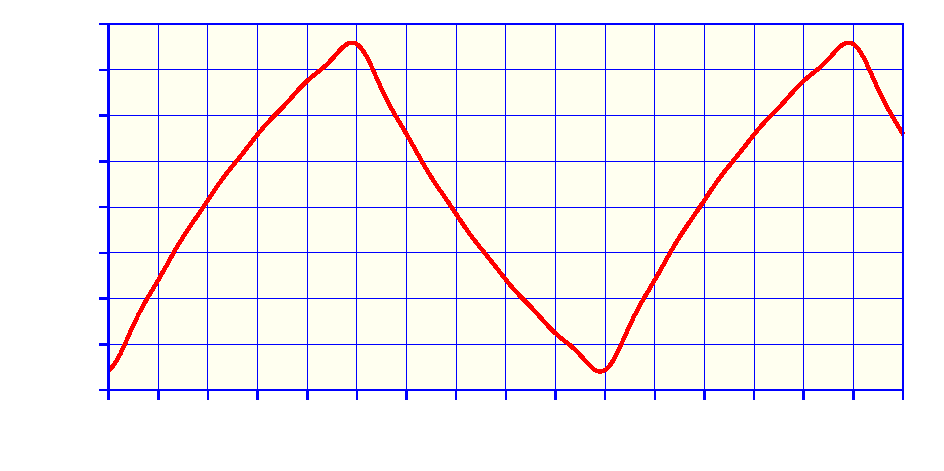
\includegraphics{Cap-Fourier-Exemple-Corrent}}%
    \gplfronttext
  \end{picture}%
\endgroup

    \end{center}

    Calculem a continuació el valor eficaç $I$ del corrent:
    \[\begin{split}
        I &= \sqrt{\left(\tfrac{\num{0,7724}}{\sqrt{2}}\si{\,A}\right)^2 +
            \left(\tfrac{\num{0,0896}}{\sqrt{2}}\si{\,A}\right)^2 +
            \left(\tfrac{\num{0,0324}}{\sqrt{2}}\si{\,A}\right)^2 +
            \left(\tfrac{\num{0,0165}}{\sqrt{2}}\si{\,A}\right)^2 +
            \left(\tfrac{\num{0,0100}}{\sqrt{2}}\si{\,A}\right)^2 +
            \left(\tfrac{\num{0,0067}}{\sqrt{2}}\si{\,A}\right)^2 + \cdots}
            \,\approx \\[1ex]
            &\approx \SI{0,5505}{A}
    \end{split}\]

    Finalment, la potència $P$ dissipada en la resistència serà:
    \[
        P = R I^2 \approx \SI{10}{\ohm} \times (\SI{0,5505}{A})^2 =
        \SI{3,03}{W}
    \]

    Aquest valor també es pot calcular a partir de l'equació
    \eqref{eq:pot_fu}; la potència així calculada correspon a la
    potència activa cedida per la font de tensió, i donat que la
    resistència $R$ és l'únic component del circuit que en consumeix,
    aquest mètode ens proporcionarà el mateix resultat. Utilitzant els sis primers termes  de les
    expansions en sèrie de Fourier de la tensió $u(t)$ i del corrent
    $i(t)$, calculats anteriorment, tenim:

    \[\begin{split}
        P &\approx U_1 I_1 \cos\varphi_1 +  U_3 I_3 \cos\varphi_3 +
         U_5 I_5 \cos\varphi_5 + U_7 I_7 \cos\varphi_7 +
         U_9 I_9 \cos\varphi_9 + U_{11} I_{11} \cos\varphi_{11} = {}\\[0.7ex]
        &= \frac{80}{\piup\times\sqrt{2}}\si{\,V} \times
        \frac{\num{0,7724}}{\sqrt{2}}\si{\,A} \times \cos \num{1,2626} +
        \frac{80}{3\times\piup\times\sqrt{2}}\si{\,V} \times
        \frac{\num{0,0896}}{\sqrt{2}}\si{\,A} \times \cos \num{1,4651} + {} \\[0.7ex]
        &+ \frac{80}{5\times\piup\times\sqrt{2}}\si{\,V} \times
        \frac{\num{0,0324}}{\sqrt{2}}\si{\,A} \times \cos \num{1,5072} +
        \frac{80}{7\times\piup\times\sqrt{2}}\si{\,V} \times
        \frac{\num{0,0165}}{\sqrt{2}}\si{\,A} \times \cos \num{1,5254} + {}\\[0.7ex]
        &+ \frac{80}{9\times\piup\times\sqrt{2}}\si{\,V} \times
        \frac{\num{0,0100}}{\sqrt{2}}\si{\,A} \times \cos \num{1,5354} +
        \frac{80}{11\times\piup\times\sqrt{2}}\si{\,V} \times
        \frac{\num{0,0067}}{\sqrt{2}}\si{\,A} \times \cos \num{1,5419}= {}\\[0.7ex]
        &= \SI{3,03}{W}
    \end{split}\]

    En la resolució d'aquest exemple hem emprat únicament els sis
    primers termes de les sèries de Fourier de la tensió i del corrent,
    no obstant, el valor  obtingut de la potència ha de ser prou precís, ja que
    els valors de pic dels termes de la sèrie del corrent disminueixen de
    valor ràpidament.

    Refarem a continuació els càlculs utilitzant més termes, amb l'ajut
    del programa
    \emph{Mathematica®}.   \index{Mathematica@\emph{Mathematica®}}

    Definim en primer lloc el valor de pic de cada
     terme de la tensió i el valor del mòdul de la impedància corresponent,
    calculem a continuació els cent primers termes  del corrent de pic (component fonamental més components harmòniques 3, 5, ..., 197 i 199), i
    per acabar calculem el valor eficaç del corrent i la potència:

    \hspace{1cm}\funsfbs{In[1]:= Upic[n\_] = 80 / (\mathsfbs{\piup} (2 n - 1));}

    \hspace{1cm}\funsfbs{In[2]:= Z[n\_] = Abs[10 + i (2 n - 1) 200 \mathsfbs{\piup} 50 \mathsfbs{10^{-3}}];}

    \hspace{1cm}\funsfbs{In[3]:= Ipic = Table[Upic[n] / Z[n], \{n, 1, 100\}];}

    \hspace{1cm}\funsfbs{In[4]:= Irms = \mathsfbs{\sqrt{Apply[Plus, (Ipic / \mathsfbs{\sqrt{2}})\mathsfbs{\phantom{}^2}]}} // N}

    \hspace{1cm}\funsfbs{Out[4]:= 0.550511}

    \hspace{1cm}\funsfbs{In[5]:= P = 10 \mathsfbs{Irms^2}}

    \hspace{1cm}\funsfbs{Out[5]:= 3.03063}\newline

    També podem fer aquests càlculs amb el programa
    \emph{MATLAB®}, tal com es veu a continuació:
    \index{MATLAB@\emph{MATLAB®}}


    \hspace{1cm}\funsfbs{> > Upic = 80 ./ (pi*(2*[1:1:100]-1));}

    \hspace{1cm}\funsfbs{> > Z = abs(10 + i*(2*[1:1:100]-1)*200*pi*50*1e-3);}

    \hspace{1cm}\funsfbs{> > Ipic = Upic ./ Z;}

    \hspace{1cm}\funsfbs{> > Irms = sqrt(sum((Ipic ./ sqrt(2)).\^{}2))}

    \hspace{1cm}\funsfbs{Irms =}

    \hspace{1cm}\funsfbs{\phantom{Irms }0.5505}

    \hspace{1cm}\funsfbs{> > P = 10*Irms\^{}2}

    \hspace{1cm}\funsfbs{P =}

    \hspace{1cm}\funsfbs{\phantom{Irms }3.0306}\newline


    Per acabar farem aquests càlculs amb la calculadora \emph{HP Prime}.
    \index{HP Prime!exemples} Els passos a seguir són els següents:

    \begin{dingautolist}{'312}

        \item En primer lloc, premem la tecla 
\includegraphics{HPPrime-Apps.pdf} i seleccionem l'aplicació \funsfbs{Function}.

             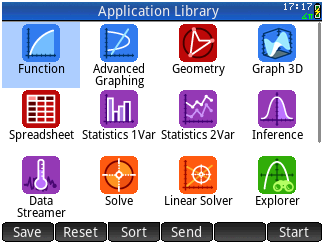
\includegraphics{Cap-Fourier-HPP1.png}

        \item Tot seguit entrem en els camps \funsfbs{F1(X)}, \funsfbs{F2(X)}, \funsfbs{F3(X)} i \funsfbs{F4(X)}, les funcions que defineixen el valor de pic de cada terme de la tensió,  el valor del mòdul de cada terme de la impedància,  la intensitat eficaç i la potència respectivament.

            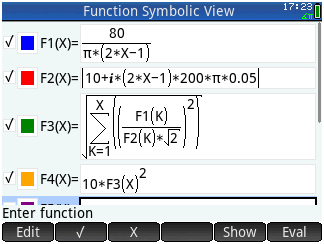
\includegraphics{Cap-Fourier-HPP2.png}

        \item  A continuació premem les tecles 
\includegraphics{HPPrime-Shift.pdf} 
\includegraphics{HPPrime-Num.pdf}, i ajustem els paràmetres de la visualització numèrica \funsfbs{Num Start} i \funsfbs{Num Step}, a \funsfbs{95} i \funsfbs{1} respectivament.

            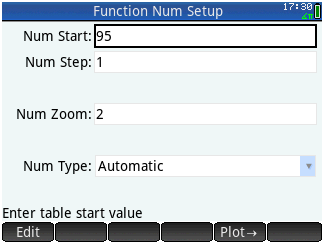
\includegraphics{Cap-Fourier-HPP3.png}

        \item Per acabar premem la tecla 
\includegraphics{HPPrime-Num.pdf}; podem veure en la columna \funsfbs{F4} i la fila corresponent a \funsfbs{X=100}, el valor calculat de la potència.

            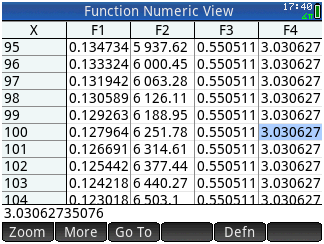
\includegraphics{Cap-Fourier-HPP4.png}

    \end{dingautolist}

    Finalment, aprofitant la potència de càlcul d'aquests programes, tornem a dibuixar les gràfiques de la tensió $u(t)$ i del corrent $i(t)$ utilitzant els trenta primers termes de les seves expansions en sèrie de Fourier (components fonamentals més components harmòniques 3, 5, ..., 57 i 59):
    \vspace{-2mm}
    \begin{center}
      % GNUPLOT: LaTeX picture with Postscript
\begingroup
  \makeatletter
  \providecommand\color[2][]{%
    \GenericError{(gnuplot) \space\space\space\@spaces}{%
      Package color not loaded in conjunction with
      terminal option `colourtext'%
    }{See the gnuplot documentation for explanation.%
    }{Either use 'blacktext' in gnuplot or load the package
      color.sty in LaTeX.}%
    \renewcommand\color[2][]{}%
  }%
  \providecommand\includegraphics[2][]{%
    \GenericError{(gnuplot) \space\space\space\@spaces}{%
      Package graphicx or graphics not loaded%
    }{See the gnuplot documentation for explanation.%
    }{The gnuplot epslatex terminal needs graphicx.sty or graphics.sty.}%
    \renewcommand\includegraphics[2][]{}%
  }%
  \providecommand\rotatebox[2]{#2}%
  \@ifundefined{ifGPcolor}{%
    \newif\ifGPcolor
    \GPcolortrue
  }{}%
  \@ifundefined{ifGPblacktext}{%
    \newif\ifGPblacktext
    \GPblacktexttrue
  }{}%
  % define a \g@addto@macro without @ in the name:
  \let\gplgaddtomacro\g@addto@macro
  % define empty templates for all commands taking text:
  \gdef\gplbacktext{}%
  \gdef\gplfronttext{}%
  \makeatother
  \ifGPblacktext
    % no textcolor at all
    \def\colorrgb#1{}%
    \def\colorgray#1{}%
  \else
    % gray or color?
    \ifGPcolor
      \def\colorrgb#1{\color[rgb]{#1}}%
      \def\colorgray#1{\color[gray]{#1}}%
      \expandafter\def\csname LTw\endcsname{\color{white}}%
      \expandafter\def\csname LTb\endcsname{\color{black}}%
      \expandafter\def\csname LTa\endcsname{\color{black}}%
      \expandafter\def\csname LT0\endcsname{\color[rgb]{1,0,0}}%
      \expandafter\def\csname LT1\endcsname{\color[rgb]{0,1,0}}%
      \expandafter\def\csname LT2\endcsname{\color[rgb]{0,0,1}}%
      \expandafter\def\csname LT3\endcsname{\color[rgb]{1,0,1}}%
      \expandafter\def\csname LT4\endcsname{\color[rgb]{0,1,1}}%
      \expandafter\def\csname LT5\endcsname{\color[rgb]{1,1,0}}%
      \expandafter\def\csname LT6\endcsname{\color[rgb]{0,0,0}}%
      \expandafter\def\csname LT7\endcsname{\color[rgb]{1,0.3,0}}%
      \expandafter\def\csname LT8\endcsname{\color[rgb]{0.5,0.5,0.5}}%
    \else
      % gray
      \def\colorrgb#1{\color{black}}%
      \def\colorgray#1{\color[gray]{#1}}%
      \expandafter\def\csname LTw\endcsname{\color{white}}%
      \expandafter\def\csname LTb\endcsname{\color{black}}%
      \expandafter\def\csname LTa\endcsname{\color{black}}%
      \expandafter\def\csname LT0\endcsname{\color{black}}%
      \expandafter\def\csname LT1\endcsname{\color{black}}%
      \expandafter\def\csname LT2\endcsname{\color{black}}%
      \expandafter\def\csname LT3\endcsname{\color{black}}%
      \expandafter\def\csname LT4\endcsname{\color{black}}%
      \expandafter\def\csname LT5\endcsname{\color{black}}%
      \expandafter\def\csname LT6\endcsname{\color{black}}%
      \expandafter\def\csname LT7\endcsname{\color{black}}%
      \expandafter\def\csname LT8\endcsname{\color{black}}%
    \fi
  \fi
    \setlength{\unitlength}{0.0500bp}%
    \ifx\gptboxheight\undefined%
      \newlength{\gptboxheight}%
      \newlength{\gptboxwidth}%
      \newsavebox{\gptboxtext}%
    \fi%
    \setlength{\fboxrule}{0.5pt}%
    \setlength{\fboxsep}{1pt}%
\begin{picture}(9060.00,4520.00)%
    \gplgaddtomacro\gplbacktext{%
      \colorrgb{0.00,0.00,0.00}%%
      \put(655,787){\makebox(0,0)[r]{\strut{}-25}}%
      \colorrgb{0.00,0.00,0.00}%%
      \put(655,1138){\makebox(0,0)[r]{\strut{}-20}}%
      \colorrgb{0.00,0.00,0.00}%%
      \put(655,1490){\makebox(0,0)[r]{\strut{}-15}}%
      \colorrgb{0.00,0.00,0.00}%%
      \put(655,1841){\makebox(0,0)[r]{\strut{}-10}}%
      \colorrgb{0.00,0.00,0.00}%%
      \put(655,2192){\makebox(0,0)[r]{\strut{}-5}}%
      \colorrgb{0.00,0.00,0.00}%%
      \put(655,2544){\makebox(0,0)[r]{\strut{} 0}}%
      \colorrgb{0.00,0.00,0.00}%%
      \put(655,2895){\makebox(0,0)[r]{\strut{} 5}}%
      \colorrgb{0.00,0.00,0.00}%%
      \put(655,3246){\makebox(0,0)[r]{\strut{} 10}}%
      \colorrgb{0.00,0.00,0.00}%%
      \put(655,3597){\makebox(0,0)[r]{\strut{} 15}}%
      \colorrgb{0.00,0.00,0.00}%%
      \put(655,3949){\makebox(0,0)[r]{\strut{} 20}}%
      \colorrgb{0.00,0.00,0.00}%%
      \put(655,4300){\makebox(0,0)[r]{\strut{} 25}}%
      \colorrgb{0.00,0.00,0.00}%%
      \put(839,481){\makebox(0,0){\strut{}$0$}}%
      \colorrgb{0.00,0.00,0.00}%%
      \put(1273,481){\makebox(0,0){\strut{}$1$}}%
      \colorrgb{0.00,0.00,0.00}%%
      \put(1707,481){\makebox(0,0){\strut{}$2$}}%
      \colorrgb{0.00,0.00,0.00}%%
      \put(2141,481){\makebox(0,0){\strut{}$3$}}%
      \colorrgb{0.00,0.00,0.00}%%
      \put(2575,481){\makebox(0,0){\strut{}$4$}}%
      \colorrgb{0.00,0.00,0.00}%%
      \put(3009,481){\makebox(0,0){\strut{}$5$}}%
      \colorrgb{0.00,0.00,0.00}%%
      \put(3443,481){\makebox(0,0){\strut{}$6$}}%
      \colorrgb{0.00,0.00,0.00}%%
      \put(3877,481){\makebox(0,0){\strut{}$7$}}%
      \colorrgb{0.00,0.00,0.00}%%
      \put(4311,481){\makebox(0,0){\strut{}$8$}}%
      \colorrgb{0.00,0.00,0.00}%%
      \put(4745,481){\makebox(0,0){\strut{}$9$}}%
      \colorrgb{0.00,0.00,0.00}%%
      \put(5179,481){\makebox(0,0){\strut{}$10$}}%
      \colorrgb{0.00,0.00,0.00}%%
      \put(5613,481){\makebox(0,0){\strut{}$11$}}%
      \colorrgb{0.00,0.00,0.00}%%
      \put(6047,481){\makebox(0,0){\strut{}$12$}}%
      \colorrgb{0.00,0.00,0.00}%%
      \put(6481,481){\makebox(0,0){\strut{}$13$}}%
      \colorrgb{0.00,0.00,0.00}%%
      \put(6915,481){\makebox(0,0){\strut{}$14$}}%
      \colorrgb{0.00,0.00,0.00}%%
      \put(7349,481){\makebox(0,0){\strut{}$15$}}%
      \colorrgb{0.00,0.00,0.00}%%
      \put(7783,481){\makebox(0,0){\strut{}$16$}}%
      \colorrgb{0.00,0.00,0.00}%%
      \put(7967,787){\makebox(0,0)[l]{\strut{}-1,25}}%
      \colorrgb{0.00,0.00,0.00}%%
      \put(7967,1138){\makebox(0,0)[l]{\strut{}-1,00}}%
      \colorrgb{0.00,0.00,0.00}%%
      \put(7967,1490){\makebox(0,0)[l]{\strut{}-0,75}}%
      \colorrgb{0.00,0.00,0.00}%%
      \put(7967,1841){\makebox(0,0)[l]{\strut{}-0,50}}%
      \colorrgb{0.00,0.00,0.00}%%
      \put(7967,2192){\makebox(0,0)[l]{\strut{}-0,25}}%
      \colorrgb{0.00,0.00,0.00}%%
      \put(7967,2544){\makebox(0,0)[l]{\strut{} 0,00}}%
      \colorrgb{0.00,0.00,0.00}%%
      \put(7967,2895){\makebox(0,0)[l]{\strut{} 0,25}}%
      \colorrgb{0.00,0.00,0.00}%%
      \put(7967,3246){\makebox(0,0)[l]{\strut{} 0,50}}%
      \colorrgb{0.00,0.00,0.00}%%
      \put(7967,3597){\makebox(0,0)[l]{\strut{} 0,75}}%
      \colorrgb{0.00,0.00,0.00}%%
      \put(7967,3949){\makebox(0,0)[l]{\strut{} 1,00}}%
      \colorrgb{0.00,0.00,0.00}%%
      \put(7967,4300){\makebox(0,0)[l]{\strut{} 1,25}}%
    }%
    \gplgaddtomacro\gplfronttext{%
      \csname LTb\endcsname%%
      \put(207,2543){\rotatebox{-270}{\makebox(0,0){\strut{}$u(t)\,  / \,\si{V}$}}}%
      \csname LTb\endcsname%%
      \put(8706,2543){\rotatebox{-270}{\makebox(0,0){\strut{}$i(t)\,  / \,\si{A}$}}}%
      \csname LTb\endcsname%%
      \put(4311,153){\makebox(0,0){\strut{}$t\, / \,\si{ms}$}}%
      \csname LTb\endcsname%%
      \put(4311,4191){\makebox(0,0){\strut{}}}%
      \csname LTb\endcsname%%
      \put(4311,4300){\makebox(0,0){\strut{}}}%
      \csname LTb\endcsname%%
      \put(4310,4049){\makebox(0,0){\strut{}}}%
      \csname LTb\endcsname%%
      \put(4330,3967){\makebox(0,0)[l]{\strut{}$u(t)$}}%
      \csname LTb\endcsname%%
      \put(4330,3639){\makebox(0,0)[l]{\strut{}$i(t)$}}%
    }%
    \gplbacktext
    \put(0,0){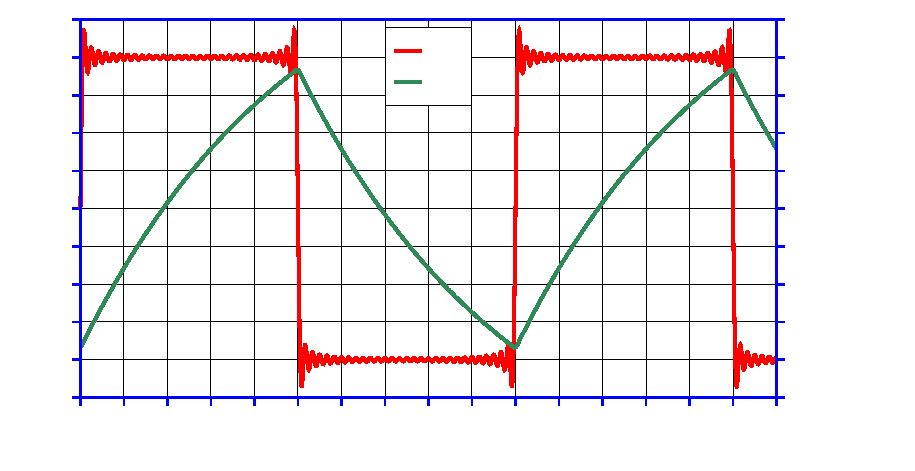
\includegraphics{Cap-Fourier-Exemple-Tensio-Corrent}}%
    \gplfronttext
  \end{picture}%
\endgroup

    \end{center}

    Per acabar, trobarem el corrent $i(t)$ utilitzant les equacions del corrent que circula en un circuit R-L, desenvolupades en la secció \vref{sec:RL-carrega}. Cal tenir en compte que aquest mètode ens dona una evolució temporal precisa, la qual comença amb el règim transitori i va evolucionant cap al règim permanent; el mètode del desenvolupament en sèrie de Fourier, en canvi, ens proporciona només el règim permanent.

    Per  poder comparar els dos mètodes haurem de veure  ara com evoluciona el corrent $i(t)$ en un període més llarg de temps, per tal d'arribar al règim permanent; suposarem que el corrent inicial és nul, i per tant usarem l'equació \eqref{eq:RL-i-carrega} per a $\SI{0}{ms} \leq t < \SI{5}{ms}$, i l'equació \eqref{eq:RL-i-carrega-ini} per a $t \geq \SI{5}{ms}$.

    La constant de temps d'aquest circuit és: $\tau = \dfrac{\SI{50}{mH}}{\SI{10}{\ohm}} = \SI{5}{ms}$.


    Es donen a continuació, les equacions dels corrents que existeixen en cadascun dels intervals de \SI{5}{ms}, compresos entre 0 ms i 35 ms. La formació d'aquestes equacions es pot veure de forma més detallada en l'exemple \vref{ex:carrega-descarrega-RL}:
    \begin{align*}
      \phantom{0}\SI{0}{ms} \leq t < \phantom{0}\SI{5}{ms}  & \quad\rightarrow\quad i_1(t) = 2 - 2 \,\eu^{-t/0,005} \\
      \phantom{0}\SI{5}{ms} \leq t < \SI{10}{ms} & \quad\rightarrow\quad i_2(t) = -2 - \big[-2 - i_1(0,005)\big]\, \eu^{-(t-0,005)/0,005}  \\
      \SI{10}{ms}\leq t < \SI{15}{ms} & \quad\rightarrow\quad i_3(t) = 2 - \big[2 - i_2(0,010)\big]\, \eu^{-(t-0,010)/0,005} \\
      \SI{15}{ms} \leq t < \SI{20}{ms} & \quad\rightarrow\quad i_4(t) = -2 - \big[-2 - i_3(0,015)\big]\, \eu^{-(t-0,015)/0,005}  \\
      \SI{20}{ms}\leq t < \SI{25}{ms} & \quad\rightarrow\quad i_5(t) = 2 - \big[2 - i_4(0,020)\big]\, \eu^{-(t-0,020)/0,005} \\
      \SI{25}{ms} \leq t < \SI{30}{ms} & \quad\rightarrow\quad i_6(t) = -2 - \big[-2 - i_5(0,025)\big]\, \eu^{-(t-0,025)/0,005}  \\
      \SI{30}{ms}\leq t < \SI{35}{ms} & \quad\rightarrow\quad i_7(t) = 2 - \big[2 - i_6(0,030)\big]\, \eu^{-(t-0,030)/0,005}
    \end{align*}

    Es representa a continuació la gràfica del corrent $i(t)$, format pels corrents $i_1(t)$ a $i_7(t)$, conjuntament amb la gràfica de la tensió $u(t)$:
    \begin{center}
      % GNUPLOT: LaTeX picture with Postscript
\begingroup
  \makeatletter
  \providecommand\color[2][]{%
    \GenericError{(gnuplot) \space\space\space\@spaces}{%
      Package color not loaded in conjunction with
      terminal option `colourtext'%
    }{See the gnuplot documentation for explanation.%
    }{Either use 'blacktext' in gnuplot or load the package
      color.sty in LaTeX.}%
    \renewcommand\color[2][]{}%
  }%
  \providecommand\includegraphics[2][]{%
    \GenericError{(gnuplot) \space\space\space\@spaces}{%
      Package graphicx or graphics not loaded%
    }{See the gnuplot documentation for explanation.%
    }{The gnuplot epslatex terminal needs graphicx.sty or graphics.sty.}%
    \renewcommand\includegraphics[2][]{}%
  }%
  \providecommand\rotatebox[2]{#2}%
  \@ifundefined{ifGPcolor}{%
    \newif\ifGPcolor
    \GPcolortrue
  }{}%
  \@ifundefined{ifGPblacktext}{%
    \newif\ifGPblacktext
    \GPblacktexttrue
  }{}%
  % define a \g@addto@macro without @ in the name:
  \let\gplgaddtomacro\g@addto@macro
  % define empty templates for all commands taking text:
  \gdef\gplbacktext{}%
  \gdef\gplfronttext{}%
  \makeatother
  \ifGPblacktext
    % no textcolor at all
    \def\colorrgb#1{}%
    \def\colorgray#1{}%
  \else
    % gray or color?
    \ifGPcolor
      \def\colorrgb#1{\color[rgb]{#1}}%
      \def\colorgray#1{\color[gray]{#1}}%
      \expandafter\def\csname LTw\endcsname{\color{white}}%
      \expandafter\def\csname LTb\endcsname{\color{black}}%
      \expandafter\def\csname LTa\endcsname{\color{black}}%
      \expandafter\def\csname LT0\endcsname{\color[rgb]{1,0,0}}%
      \expandafter\def\csname LT1\endcsname{\color[rgb]{0,1,0}}%
      \expandafter\def\csname LT2\endcsname{\color[rgb]{0,0,1}}%
      \expandafter\def\csname LT3\endcsname{\color[rgb]{1,0,1}}%
      \expandafter\def\csname LT4\endcsname{\color[rgb]{0,1,1}}%
      \expandafter\def\csname LT5\endcsname{\color[rgb]{1,1,0}}%
      \expandafter\def\csname LT6\endcsname{\color[rgb]{0,0,0}}%
      \expandafter\def\csname LT7\endcsname{\color[rgb]{1,0.3,0}}%
      \expandafter\def\csname LT8\endcsname{\color[rgb]{0.5,0.5,0.5}}%
    \else
      % gray
      \def\colorrgb#1{\color{black}}%
      \def\colorgray#1{\color[gray]{#1}}%
      \expandafter\def\csname LTw\endcsname{\color{white}}%
      \expandafter\def\csname LTb\endcsname{\color{black}}%
      \expandafter\def\csname LTa\endcsname{\color{black}}%
      \expandafter\def\csname LT0\endcsname{\color{black}}%
      \expandafter\def\csname LT1\endcsname{\color{black}}%
      \expandafter\def\csname LT2\endcsname{\color{black}}%
      \expandafter\def\csname LT3\endcsname{\color{black}}%
      \expandafter\def\csname LT4\endcsname{\color{black}}%
      \expandafter\def\csname LT5\endcsname{\color{black}}%
      \expandafter\def\csname LT6\endcsname{\color{black}}%
      \expandafter\def\csname LT7\endcsname{\color{black}}%
      \expandafter\def\csname LT8\endcsname{\color{black}}%
    \fi
  \fi
    \setlength{\unitlength}{0.0500bp}%
    \ifx\gptboxheight\undefined%
      \newlength{\gptboxheight}%
      \newlength{\gptboxwidth}%
      \newsavebox{\gptboxtext}%
    \fi%
    \setlength{\fboxrule}{0.5pt}%
    \setlength{\fboxsep}{1pt}%
\begin{picture}(8780.00,4520.00)%
    \gplgaddtomacro\gplbacktext{%
      \colorrgb{0.00,0.00,0.00}%
      \put(595,715){\makebox(0,0)[r]{\strut{}-25}}%
      \colorrgb{0.00,0.00,0.00}%
      \put(595,1078){\makebox(0,0)[r]{\strut{}-20}}%
      \colorrgb{0.00,0.00,0.00}%
      \put(595,1441){\makebox(0,0)[r]{\strut{}-15}}%
      \colorrgb{0.00,0.00,0.00}%
      \put(595,1803){\makebox(0,0)[r]{\strut{}-10}}%
      \colorrgb{0.00,0.00,0.00}%
      \put(595,2166){\makebox(0,0)[r]{\strut{}-5}}%
      \colorrgb{0.00,0.00,0.00}%
      \put(595,2529){\makebox(0,0)[r]{\strut{} 0}}%
      \colorrgb{0.00,0.00,0.00}%
      \put(595,2892){\makebox(0,0)[r]{\strut{} 5}}%
      \colorrgb{0.00,0.00,0.00}%
      \put(595,3255){\makebox(0,0)[r]{\strut{} 10}}%
      \colorrgb{0.00,0.00,0.00}%
      \put(595,3617){\makebox(0,0)[r]{\strut{} 15}}%
      \colorrgb{0.00,0.00,0.00}%
      \put(595,3980){\makebox(0,0)[r]{\strut{} 20}}%
      \colorrgb{0.00,0.00,0.00}%
      \put(595,4343){\makebox(0,0)[r]{\strut{} 25}}%
      \colorrgb{0.00,0.00,0.00}%
      \put(762,437){\makebox(0,0){\strut{}$0$}}%
      \colorrgb{0.00,0.00,0.00}%
      \put(1717,437){\makebox(0,0){\strut{}$5$}}%
      \colorrgb{0.00,0.00,0.00}%
      \put(2671,437){\makebox(0,0){\strut{}$10$}}%
      \colorrgb{0.00,0.00,0.00}%
      \put(3626,437){\makebox(0,0){\strut{}$15$}}%
      \colorrgb{0.00,0.00,0.00}%
      \put(4581,437){\makebox(0,0){\strut{}$20$}}%
      \colorrgb{0.00,0.00,0.00}%
      \put(5536,437){\makebox(0,0){\strut{}$25$}}%
      \colorrgb{0.00,0.00,0.00}%
      \put(6490,437){\makebox(0,0){\strut{}$30$}}%
      \colorrgb{0.00,0.00,0.00}%
      \put(7445,437){\makebox(0,0){\strut{}$35$}}%
      \colorrgb{0.00,0.00,0.00}%
      \put(7612,715){\makebox(0,0)[l]{\strut{}-1,25}}%
      \colorrgb{0.00,0.00,0.00}%
      \put(7612,1078){\makebox(0,0)[l]{\strut{}-1,00}}%
      \colorrgb{0.00,0.00,0.00}%
      \put(7612,1441){\makebox(0,0)[l]{\strut{}-0,75}}%
      \colorrgb{0.00,0.00,0.00}%
      \put(7612,1803){\makebox(0,0)[l]{\strut{}-0,50}}%
      \colorrgb{0.00,0.00,0.00}%
      \put(7612,2166){\makebox(0,0)[l]{\strut{}-0,25}}%
      \colorrgb{0.00,0.00,0.00}%
      \put(7612,2529){\makebox(0,0)[l]{\strut{} 0,00}}%
      \colorrgb{0.00,0.00,0.00}%
      \put(7612,2892){\makebox(0,0)[l]{\strut{} 0,25}}%
      \colorrgb{0.00,0.00,0.00}%
      \put(7612,3255){\makebox(0,0)[l]{\strut{} 0,50}}%
      \colorrgb{0.00,0.00,0.00}%
      \put(7612,3617){\makebox(0,0)[l]{\strut{} 0,75}}%
      \colorrgb{0.00,0.00,0.00}%
      \put(7612,3980){\makebox(0,0)[l]{\strut{} 1,00}}%
      \colorrgb{0.00,0.00,0.00}%
      \put(7612,4343){\makebox(0,0)[l]{\strut{} 1,25}}%
    }%
    \gplgaddtomacro\gplfronttext{%
      \csname LTb\endcsname%
      \put(143,2529){\rotatebox{-270}{\makebox(0,0){\strut{}$u(t) / \si{V}$}}}%
      \csname LTb\endcsname%
      \put(8414,2529){\rotatebox{-270}{\makebox(0,0){\strut{}$i(t) / \si{A}$}}}%
      \csname LTb\endcsname%
      \put(4103,139){\makebox(0,0){\strut{}$t / \si{ms}$}}%
      \csname LTb\endcsname%
      \put(4103,4244){\makebox(0,0){\strut{}}}%
      \csname LTb\endcsname%
      \put(4103,4243){\makebox(0,0){\strut{}}}%
      \csname LTb\endcsname%
      \put(243,100){\makebox(0,0)[l]{\strut{}}}%
      \csname LTb\endcsname%
      \put(6987,1390){\makebox(0,0){\strut{}}}%
      \csname LTb\endcsname%
      \put(6961,1315){\makebox(0,0)[l]{\strut{}$u(t)$}}%
      \csname LTb\endcsname%
      \put(6961,1017){\makebox(0,0)[l]{\strut{}$i(t)$}}%
    }%
    \gplbacktext
    \put(0,0){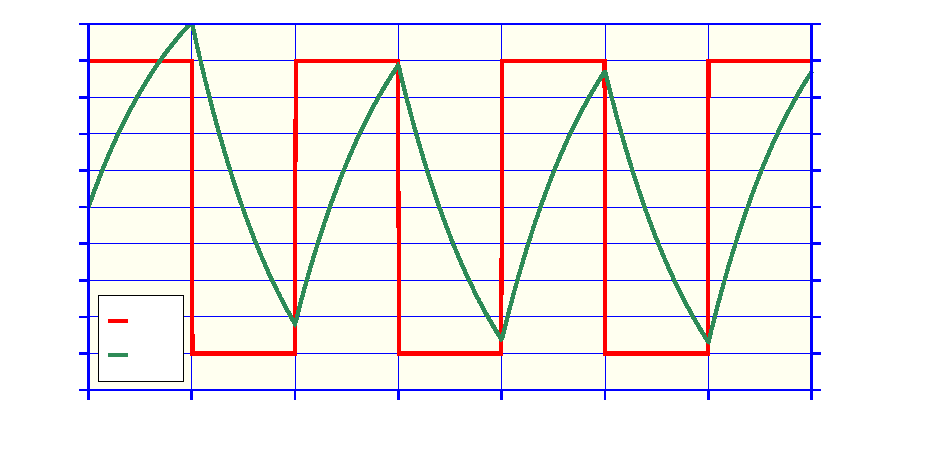
\includegraphics{Cap-Fourier-Exemple-Tensio-Corrent-RL}}%
    \gplfronttext
  \end{picture}%
\endgroup

    \end{center}

    El règim transitori inicial del corrent $i(t)$ va desapareixent progressivament, i a partir de $t=\SI{20}{ms}$ aproximadament, ja ens trobem en el règim permanent.
    A partir d'aquest instant, la forma i els valors positius i negatius màxims de $i(t)$, i la diferència temporal relativa entre $i(t)$ i $u(t)$, són equivalents als obtinguts mitjançant el mètode inicial del desenvolupament en sèrie de Fourier.

    El fet que les gràfiques de les funcions periòdiques $u(t)$ i  $i(t)$, obtingudes utilitzant el mètode del desenvolupament en sèrie de Fourier, s'hagin dibuixat començant a $t=0$ és irrellevant, ja que tal com s'ha dit,   aquest mètode ens proporciona només el règim permanent, i per tant es pot fixar a qualsevol valor l'instant del temps d'inici d'aquestes gràfiques.
\end{exemple}
